% Sketch output, version 0.3 (build 2d, Wed Apr 20 23:38:45 2011)
% Output language: PGF/TikZ,LaTeX
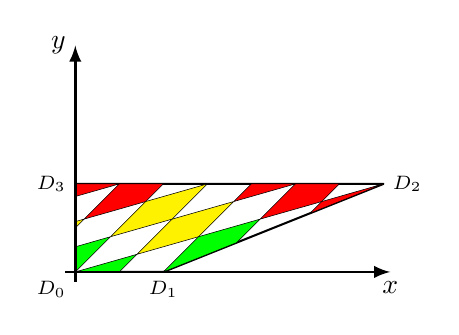
\begin{tikzpicture}[line join=round,line width=0.2pt,>=latex]
\filldraw[fill=none,line width=0.75pt](0,-12)--(1.118,-12)--(3.913,-10.882)--(0,-10.882)--cycle;
\filldraw[fill=red](2.981,-11.255)--(3.913,-10.882)--(3.13,-11.106)--cycle;
\filldraw[fill=red](2.348,-11.329)--(3.13,-11.106)--(3.354,-10.882)--(2.795,-10.882)--cycle;
\filldraw[fill=red](2.236,-10.882)--(2.012,-11.106)--(2.795,-10.882)--cycle;
\filldraw[fill=red](.559,-10.882)--(.112,-11.329)--(.894,-11.106)--(1.118,-10.882)--cycle;
\filldraw[fill=red](0,-10.882)--(0,-11.042)--(.559,-10.882)--cycle;
\filldraw[fill=yellow](.783,-11.776)--(1.565,-11.553)--(2.012,-11.106)--(1.23,-11.329)--cycle;
\filldraw[fill=yellow](.894,-11.106)--(.447,-11.553)--(1.23,-11.329)--(1.677,-10.882)--cycle;
\filldraw[fill=yellow](.112,-11.329)--(0,-11.441)--(0,-11.361)--cycle;
\filldraw[fill=green](1.118,-12)--(2.05,-11.627)--(2.348,-11.329)--(1.565,-11.553)--cycle;
\filldraw[fill=green](0,-12)--(.559,-12)--(.783,-11.776)--cycle;
\filldraw[fill=green](0,-12)--(.447,-11.553)--(0,-11.681)--cycle;
\draw[->,line width=1pt](0,-12.125)--(0,-9.125);
\draw[->,line width=1pt](-.125,-12)--(4,-12);

    \coordinate [label=below:$x$] (X) at (4,-12);
    \coordinate [label=left:$y$] (Y) at (0,-9.125);
  
    \coordinate [label=225:\scriptsize$D_0$] (p0D) at (0,-12);
    \coordinate [label=270:\scriptsize$D_1$] (p1D) at (1.118,-12);
    \coordinate [label=000:\scriptsize$D_2$] (p2D) at (3.913,-10.882);
    \coordinate [label=180:\scriptsize$D_3$] (p3D) at (0,-10.882);
  \end{tikzpicture}% End sketch output
